\section{Hands-on examples for Graph Neural Networks}

This section will contain two Notebooks that will be crucial in comprehending how GNNs are implemented.

The first exercise consists of creating a Graph Neural Network (GNN) using \texttt{torch\_geometric} to recognize whether an image, represented as a point cloud, contains a rectangle or a circle. In the second one, you will tackle a more complex custom graph problem using the Deep Graph Library (\texttt{dgl}) to build an object condensation model. 

Here are the links to the Colab Notebooks:
\begin{enumerate}
    \item \url{https://colab.research.google.com/drive/1uz9OdJsD_RcDMlxCWqvN7rPXGWk-KZ1t?usp=sharing}
    \item \url{https://colab.research.google.com/drive/1j-rmo5-ro7LkosqiKpojPYlrqdgYzfmr?usp=sharing}
\end{enumerate}

Instead of using \texttt{keras}, we will be working with the \texttt{PyTorch} library. The rationale behind this shift is flexibility: especially within the high-energy physics community, researchers frequently need to build custom architectures that deviate from standard, built-in models. PyTorch offers the granular control required to implement these novel, physics-informed architectures, making it the standard tool for professional applications. You will find the necessary documentation here: \url{https://docs.pytorch.org/docs/main/}.

Since I have to start a new page in order to input the Notebook in my LaTeX file, here is a photo of all the Slam winners of the year 2000. In order: Andre Agassi at the 2000 Australian Open (\textit{upper left}), Gustavo Kuerten at the 2000 Roland Garros (\textit{upper right}), Pete Sampras at the 2000 Wimbledon with the runner-up Pat Rafter (\textit{bottom left}) and Marat Safin at the 2000 US Open (\textit{bottom right}).  

\begin{center}
    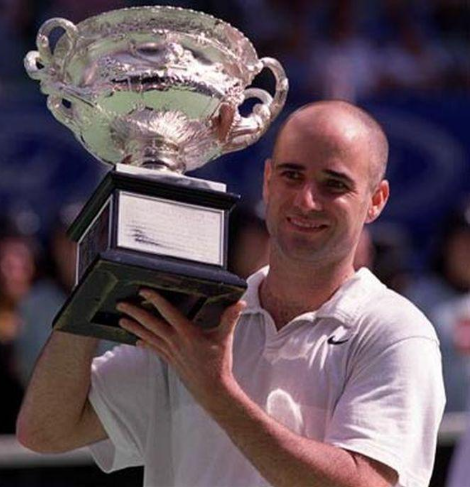
\includegraphics[width=0.3\textwidth]{figuresML/2000_agassi}
    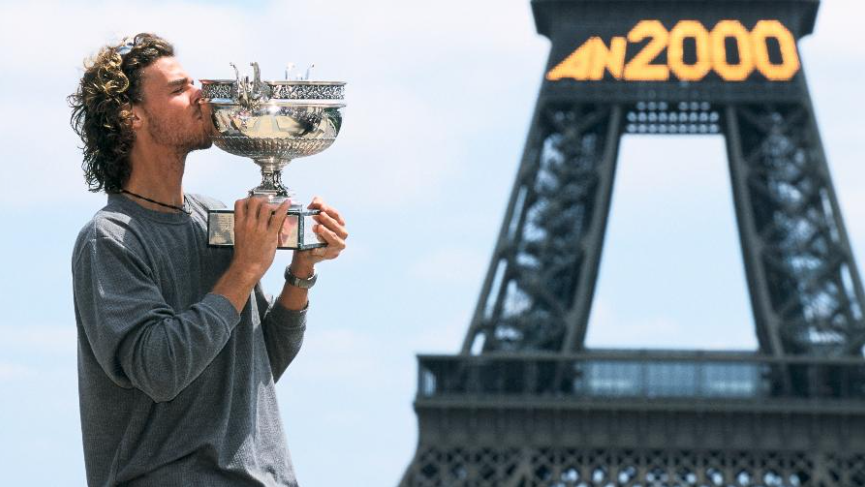
\includegraphics[width=0.5\textwidth]{figuresML/2000_kuarten}
    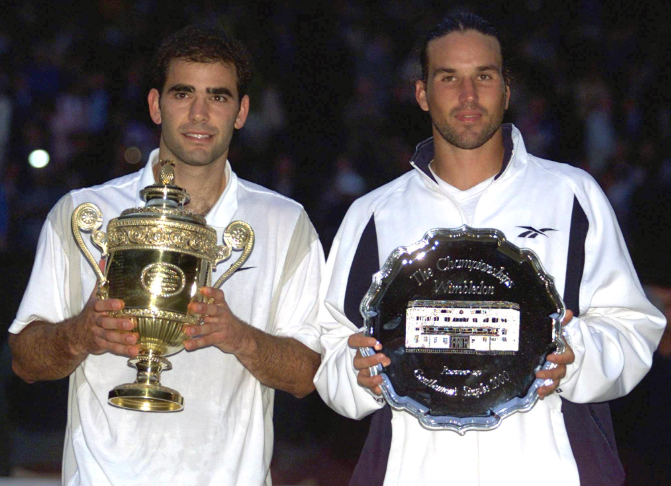
\includegraphics[width=0.5\textwidth]{figuresML/2000_sampras}
    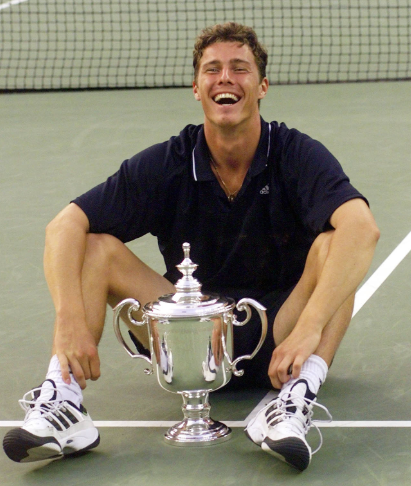
\includegraphics[width=0.3\textwidth]{figuresML/2000_safin}
\end{center}

%\includepdf[pages=-, pagecommand={\thispagestyle{plain}}]{lezioni/d_ML6a_SOL.pdf} 
%ML_5 nel mio colab

%\includepdf[pages=-, pagecommand={\thispagestyle{plain}}]{lezioni/d_ML6b_SOL.pdf}
%ML_9 nel mio colab
